\documentclass[10pt]{article}
\usepackage[utf8]{inputenc}
\usepackage{graphicx}
\usepackage[portuguese]{babel}

\title{Robôs Domésticos}
\author{André Rato[45517], Diogo Faustino[40968], José Alexandre[45223]}
\date{Maio de 2021}

\usepackage[sorting=none]{biblatex}
\bibliography{references}
\PassOptionsToPackage{hyphens}{url}
\usepackage{url}

%%% Elimiação do overlow das references %%%
\setcounter{biburllcpenalty}{7000}
\setcounter{biburlucpenalty}{8000}

\begin{document}

\maketitle
\renewcommand\abstractname{Resumo}
\begin{abstract}

Este trabalho tem como tema central "Robôs Domésticos". Com a enorme evolução que os robôs domésticos têm tido nos últimos anos, é importante perceber e entender essa evolução que passa despercebida aos nossos olhos.

Para isso, pretendemos entender melhor o que é um robô doméstico, conhecendo um pouco sobre a sua história, desde o dia em que o primeiro robô foi criado até aos dias de hoje. Para além disso, é necessário conhecer quais as vantagens e desvantagens da utilização destes robôs, sendo também necessário conhecer quais as medidas de segurança no que toca ao manuseamento e utilização destas máquinas. 

Para além dos pontos já referidos, este tema foi escolhido devido à profunda relação que a robótica tem com a inteligência artificial e ao impacto que esta tem vindo a ter no mercado financeiro mundial.

Após conhecidos todos estes aspetos, é imprescindível fazer uma pesquisa sobre alguns robôs domésticos em particular, de modo a ficar a conhecer todas as suas funções e entender como se processa a execução das tarefas para as quais são programados.


\end{abstract}
\section{Introdução}
\hspace{\parindent}O que são robôs domésticos? Como funcionam? Quais as suas funções? Quando deparadas com estas perguntas, a maioria das pessoas acaba por não conseguir responder corretamente. É com o objetivo de responder, não só a estas perguntas, mas a outras que elaborámos este artigo. 

\section{O que é um robô doméstico?}
\hspace{\parindent}Para responder a esta pergunta é necessário ter-se noção do significado dos termos "robô" e "robótica".

Um robô (ou \textit{robot}) é um dispositivo, ou grupo de dispositivos, capazes de realizar trabalhos de forma autónoma ou pré-programada \cite{robot}. São normalmente utilizados na realização de tarefas perigosas para o seres humanos.

Já a robótica é a ciência associada com o projeto, fabricação, teoria e aplicação dos robôs. Esta requer conhecimentos sobre eletrotecnia, mecânica e software. A parte eletrotécnica e de software requerem conhecimentos sobre o tipo de unidade processadora a ser utilizada (microcontroladores ou CLPs) e a parte mecânica, conhecimentos sobre cinemática, pneumática e hidráulica.

Um robô doméstico é, tal como o nome indica, um robô destinado a realizar tarefas domésticas. Para além disso, estes robôs podem ainda ser utilizados no ramo da educação, no ramo do entretenimento e no ramo da terapia.\cite{dom-rob}

Mesmo que a maioria dos robôs domésticos seja simplista, alguns estão conectados, não só a redes domésticas WiFi, mas também a ambientes inteligentes, tornando-os assim autónomos em alto grau. 


\section{História e evolução}
\hspace{\parindent}A primeira aparição de robôs deu-se na altura da Revolução Industrial, os quais foram criados para processar materiais e para criar produtos. Este evento foi um marco para a história da humanidade pois a qualidade vida do Homem melhorou bastante neste período.

Após a evolução rápida destes robôs, as pessoas começaram a usufruir das suas funcionalidades em casa, dando origem assim aos primeiros robôs domésticos. 

Nesta época existiam muitas dúvidas em relação aos robôs, pois um dos temas mais falados era o facto de os robôs se revoltarem contra os humanos. É aqui que entra o escritor Isaac Asimov que, após toda esta preocupação relativa à segurança dos robôs, idealizou três leis fundamentais para a robótica com a finalidade de controlar e limitar os comportamentos dos robôs:

\begin{itemize}
    \item \textbf{1ª Lei:} nenhum robô pode ferir um ser humano, ou por inação, que o ser humano sofra algum mal;
    \item \textbf{2ª Lei:} todos os robôs devem obedecer às ordens que são dadas pelos seres humanos, exceto se essa ordem entrar em conflito com a 1ª Lei;
    \item \textbf{3ª Lei:} qualquer robô deve proteger a sua própria existência, desde que essa proteção não entre em conflito com a 1ª e 2ª Leis.
\end{itemize}

Mais tarde, Asimov acrescentou a \textbf{"Lei Zero"}, que está acima das outras todas, e refere que nenhum robô pode causar mal à humanidade, e por omissão, permitir que a humanidade sofra algum mal.

Estas leis foram apresentadas em 1942, e se não fosse por elas, muito provavelmente não teríamos assistido a esta evolução dos robôs, pois só com elas se pôde começar a confiar neles para o nosso dia-a-dia.

Um dos primeiros robôs domésticos a ser criado chamava-se \textit{HERO}, que foi vendido durante os anos 80. Existiram quatro modelos deste robô, sendo a primeira o \textit{HERO 1}. Este modelo foi usado para educação e para conseguir responder à procura da população; já o \textit{HERO JR} foi criado para uso próprio. As últimas duas gerações foram o \textit{HERO 2000} e o \textit{Arm Trainer}. \textit{HERO 1} como máquina utilizada para educação, tinha uma sensibilidade muito boa. Conseguia reunir informação com precisão e analisá-la. Uma versão melhorada do \textit{HERO 1} foi o \textit{HERO 2000} que tinha um destaque em "programabilidade avançada" \cite{history}. O \textit{Arm Trainer} foi utilizado para a área industrial, o que permitiu controlar robôs industriais de grande escala. Nisto tudo, o melhoramento mais importante foi a passagem do \textit{HERO 1} para o \textit{HERO JR}. O \textit{HERO JR} foi o primeiro robô com um preço acessível, e com uma personalidade dinâmica. As pessoas podiam usá-lo para tocar músicas, para jogar, para acordar de manhã, para notificar sobre eventos, e podiam até vigiar a casa.

Outro protótipo de um robô doméstico foi o \textit{Topo}, que foi desenvolvido pela \textit{Androbot Inc.} em 1983. A sua linguagem de programação permitia movimentos geométricos e realizar tarefas, mas não tinha um sensor, então não podia ser considerado um robô. Para resolver este problema, a segunda e terceira geração continham um transmissor infra-vermelhos e podia ser controlado remotamente. Na sua última geração, \textit{Topo4} foi inventado, mas nunca chegou a ser fabricado e vendido ao público.

Com estes dois protótipos, os robôs domésticos tornaram-se cada vez mais acessíveis e com um preço mais apelativo. Até 2006 já existiam mais de 3 milhões de robôs em uso.

\begin{figure}[h]
\caption{Representação da evolução dos robôs domésticos}
\centering
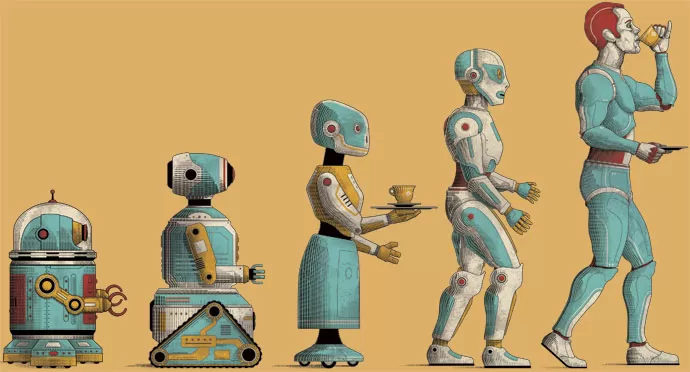
\includegraphics[width = 6cm]{img/3.png}
\label{figura:3}
\end{figure}


\section{Vantagens e desvantagens}


\subsection{Vantagens}
\hspace{\parindent}Ao longo do tempo, e com os avanços tecnológicos que temos vindo a presenciar nos últimos anos, a utilização de robôs domésticos tem-se tornado cada vez mais vantajosa.

Em casa, a robótica tem como principal objetivo facilitar a vida das famílias. Ter um robô com estas funcionalidades num ambiente com pessoas portadoras de deficiência, realizando algumas tarefas que normalmente seriam feitas pela pessoa que cuida do doente. O mesmo acontece com pessoas de idade mais avançada, pessoas estas que necessitam de algum apoio, não só físico, mas também emocional, o qual pode ser fornecido pelo robôs.

Para além disto, a existência de um robô doméstico num ambiente perigoso e inseguro pode aumentar a segurança do mesmo, tendo a possibilidade de ter câmeras automáticas que consigam distinguir pessoas, animais e objetos, fotografando aquilo que o proprietário do robô tenha definido como ameaça \cite{advantages1}.

\subsection{Desvantagens}
\hspace{\parindent}Independentemente de todo o trabalho executado pelos robôs domésticos, não nos podemos esquecer que estes não são totalmente seguros, possuindo uma vasta lista de desvantagens adjacentes à sua utilização.

Um robô apenas consegue fazer aquilo que o utilizador o ordena, ou então aquilo para o qual está programado. Deste modo, quando deparado com certas situações inesperadas, o robô não consegue improvisar, havendo assim a necessidade da existência de protocolos de segurança para proteger humanos e outros robôs \cite{advantages1}.

Embora os robôs domésticos sejam, em certos aspetos, superiores aos humanos, como por exemplo a não existência de fadiga ou a velocidade com que executam as coisas, eles são menos hábeis que os humanos, não têm cérebros poderosos que se adaptem às diversas situações, e não conseguem interpretar o que vêm tão bem como os humanos \cite{advantages2}.

Em termos monetários, mesmo que o custo inicial do robô tenha vindo a diminuir com o passar do tempo, há certos aspetos que vão tornar o custo total de um robô um pouco mais elevado que o esperado, tais como a manutenção do robô, avarias futuras que possam existir, ou a necessidade de serem programados para realizar determinadas tarefas.


\section{Inteligência artificial nos robôs domésticos}

\hspace{\parindent}A inteligência artificial (IA) é a capacidade que uma máquina tem para reproduzir competências semelhantes às humanas como é o caso do raciocínio, a aprendizagem, o planeamento e a criatividade.

A IA permite que os sistemas técnicos percebam o ambiente que os rodeia, lidem com o que percebem e resolvam problemas, agindo no sentido de alcançar um objetivo específico. O computador recebe dados (já preparados ou recolhidos através dos seus próprios sensores, por exemplo, com o uso de uma câmara), processa-os e responde.

Os sistemas de IA são capazes de adaptar o seu comportamento, até certo ponto, através de uma análise dos efeitos das ações anteriores e de um trabalho autónomo.

Algumas tecnologias de IA existem há mais de 50 anos, mas o melhor desenvolvimento da capacidade de processamento, a disponibilidade de quantidades elevadas de dados e novos algoritmos permitiram grandes progressos da IA nos últimos anos.

A inteligência artificial é considerada o ponto mais importante para a transformação digital da sociedade e tornou-se uma prioridade da União Europeia.

Estão previstas futuras aplicações que poderão trazer mudanças enormes, sendo que a IA já está presente no nosso quotidiano \cite{airobots}.


Analisando o \textit{iRobot Roomba} e o \textit{RX-V100} da \textit{Sharp Corporation}, é fácil entender como a inteligência artificial é aplicada aos robôs \cite{ai}.

\subsection{iRobot Roomba}
\hspace{\parindent}Quando a \textit{iRobot} lançou o seu primeiro aspirador de pó robótico, \textit{Roomba}, em 2002, o produto tinha recursos de IA bastante básicos, como identificar paredes e evitar escadas usando sensores embutidos. O modelo mais recente, \textit{Roomba 980},  possui recursos avançados de tomada de decisão, acionados por IA. O robô é capaz de fazer um scan do tamanho da sala, identificando obstáculos e lembrando as rotas e métodos mais eficientes.

\begin{figure}[h]
\caption{Fotografia do \textit{iRobot Roomba}}
\centering
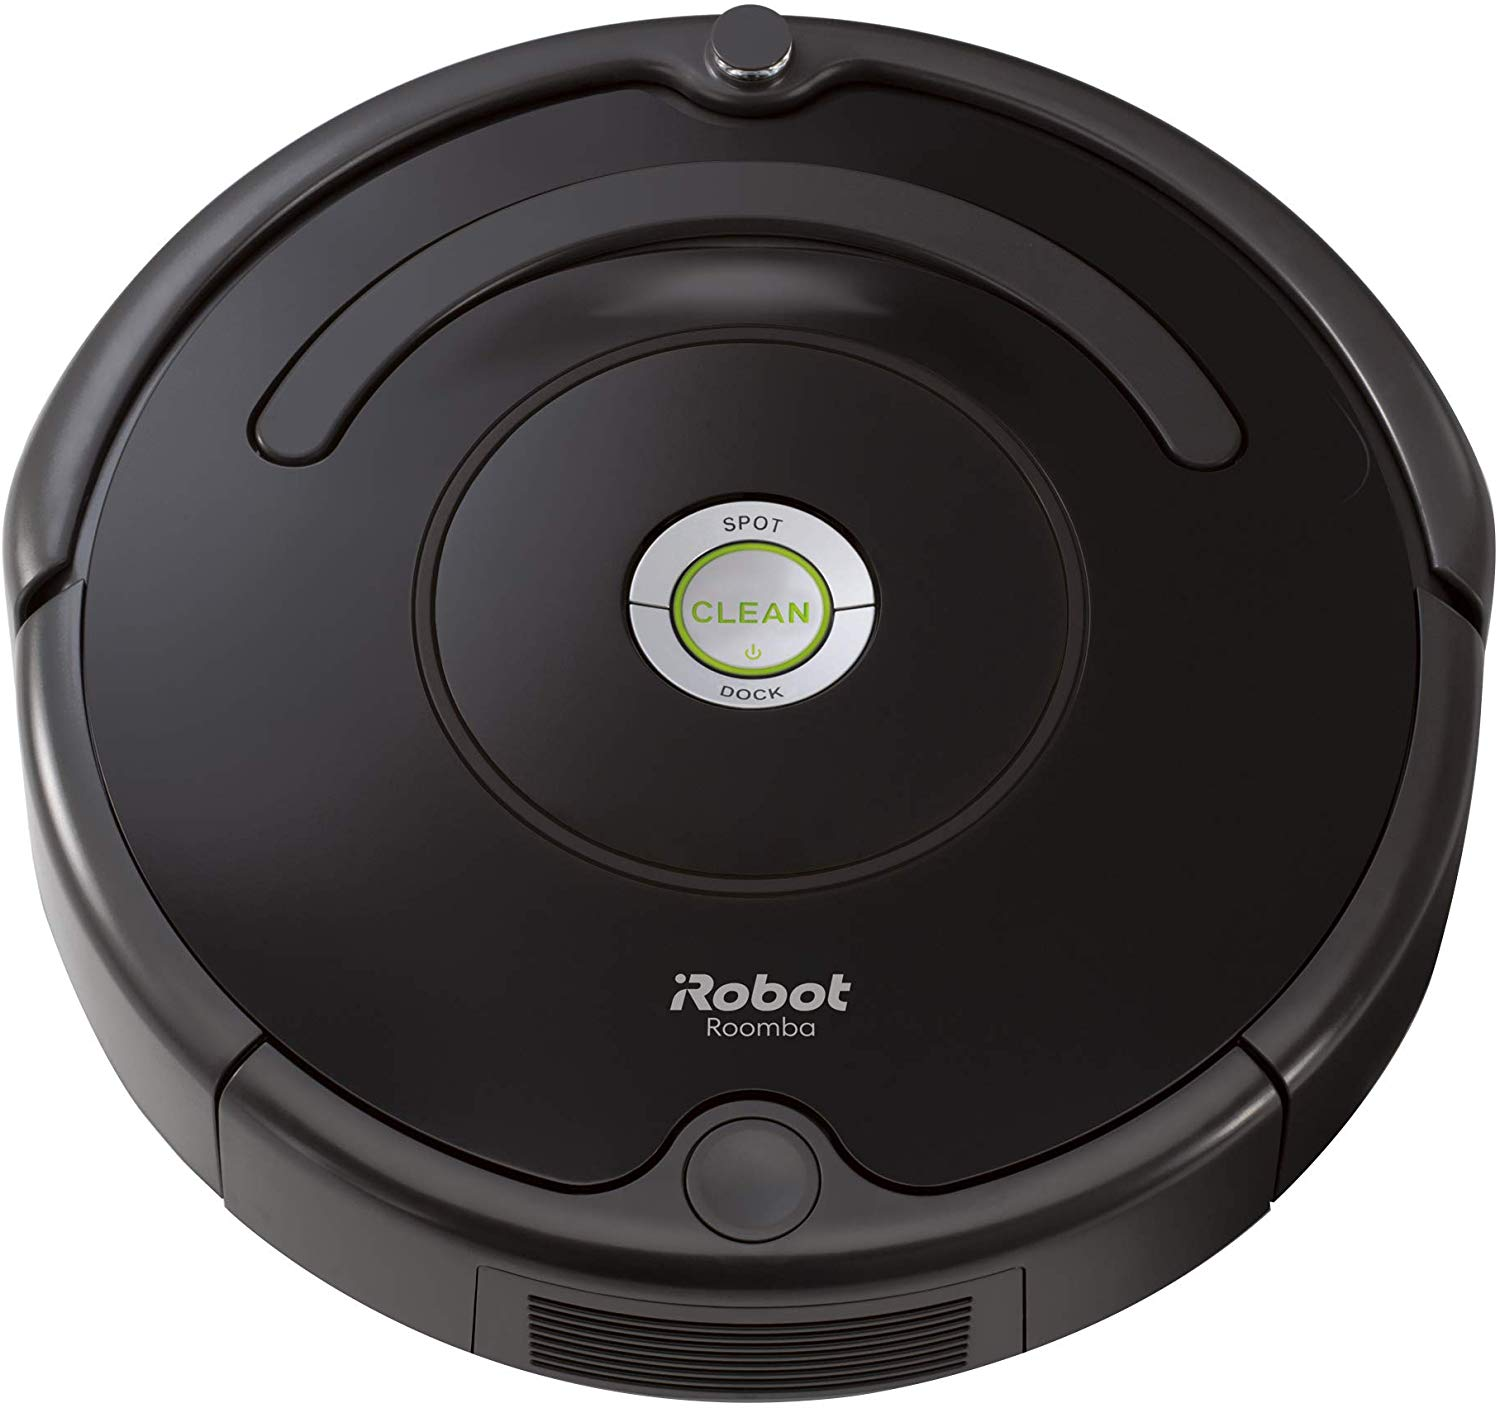
\includegraphics[width = 4cm]{img/5.1.jpg}
\label{figura:5.1}
\end{figure}

\subsection{RX-V100 da Sharp Corporation}

\hspace{\parindent}O \textit{RX-V100} é um robô de limpeza integrado com um mecanismo IA de reconhecimento de voz para permitir a realização de tarefas, tais como relatar o estado atual do robô por meio de uma combinação de luzes e mensagens faladas. Por exemplo, quando um utilizador dá um comando de voz ao robô para “Limpar”, o \textit{RX-V100} usa voz IA para responder, “Tudo bem” e “balança” para reconhecer o comando. De seguida, começa a limpeza no modo automático. Além disso, o produto vem com um conjunto de mensagens e respostas predefinidas para simular conversas simples, como “Bom dia” ou “Como está?”

\begin{figure}[h]
\caption{Fotografia do \textit{RX-V100}}
\centering
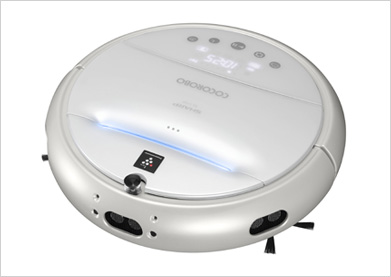
\includegraphics[width = 4cm]{img/5.2.jpg}
\label{figura:5.2}
\end{figure}

\section{Influência da robótica no mercado financeiro}

\hspace{\parindent}O mercado de robôs domésticos deve registrar um TCAC (Taxa de Crescimento Anual Composta) de 20,5\% ao longo do período de previsão (2021 - 2026). De acordo com a \textit{International Federation of Robotic Report 2019}, espera-se que as vendas unitárias de robôs domésticos aumentem 46\% em média por ano, com mais de 55 milhões de unidades vendidas em 2022. Além disso, os valores de venda dos robôs domésticos aumentaram em 15\% para 3,7 mil milhões de euros. 

As inovações tecnológicas, no que diz respeito à cognição, interação e manipulação, tornaram a robótica doméstica mais atraente. Tecnologia e outros fornecedores de componentes têm sido fundamentais para o avanço do ecossistema robótico. Por exemplo, em abril de 2019, investigadores da Universidade da Califórnia desenvolveram um robô que usa inteligência artificial (IA) para realizar tarefas humanas intrincadas, como ajudar a dobrar roupas ou fazer uma chávena de café. 

O aumento da penetração da automação em eletrodomésticos, o aumento dos custos de mão de obra e as crescentes preocupações com a segurança estão a impulsionar a procura por robôs domésticos em todo o mundo. 

Com o crescimento crescente do conceito de casa inteligente, o robô pode desempenhar um papel crucial no ecossistema de casa inteligente. Por exemplo, em 2019, Temi, uma empresa responsável por um dos maiores websites de transcrições de áudio para texto \cite{temi}, fez parceria com a Amazon Alexa para projetar robôs inteligentes, móveis e pessoais movidos a IA. A Samsung e a LG Electronics estão a investir extensivamente no desenvolvimento e lançamento de novos produtos robóticos domésticos. Por exemplo, a Jibo está desenvolvendo robôs sociais para integração na vida doméstica para companheiros interativos. Observando o potencial do mercado, as startups que oferecem soluções de robôs domésticos também estão a atrair financiamento de investidores internacionais. No entanto, o alto custo do equipamento está limitando a taxa de adoção de robôs domésticos \cite{market}.

\begin{figure}[h]
\caption{Venda de Robôs Domésticos entre 2016 e 2021}
\centering
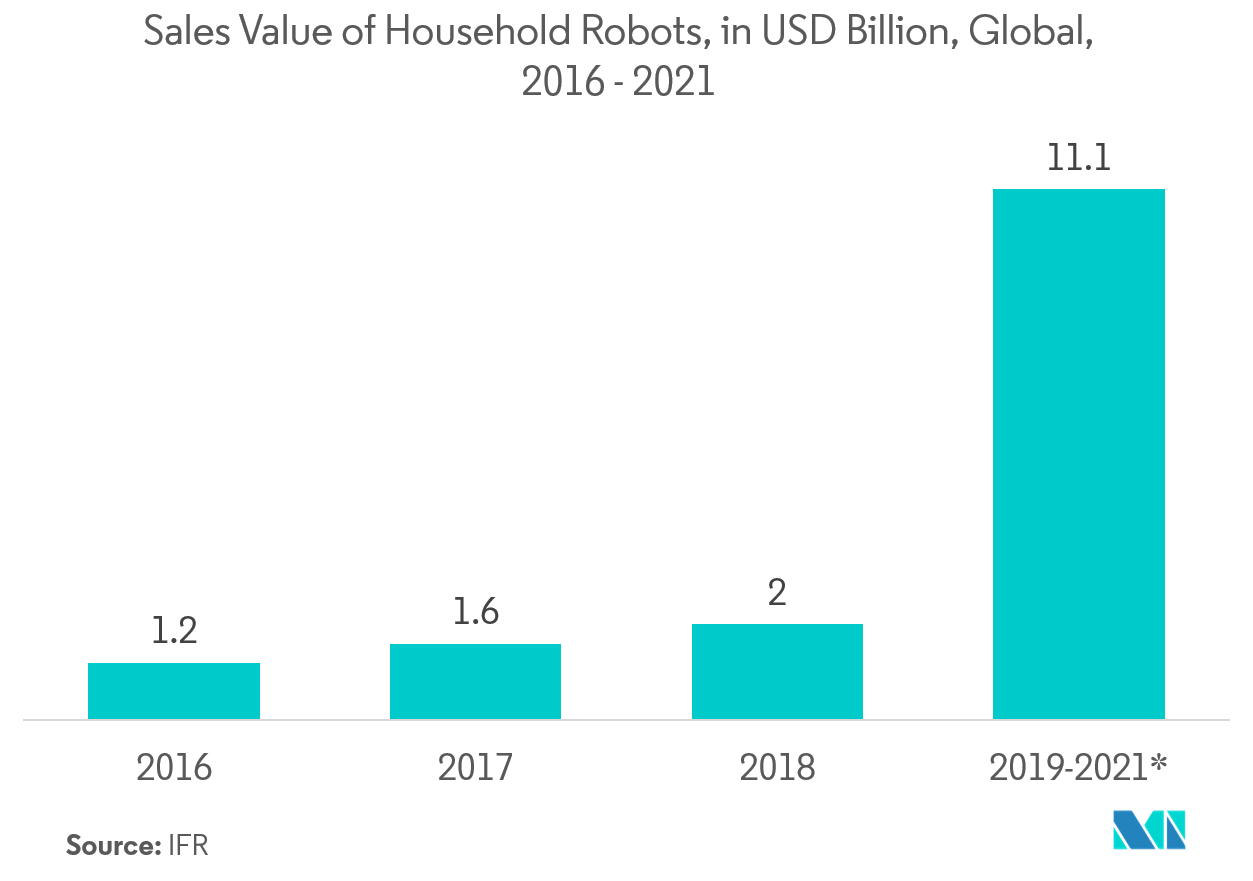
\includegraphics[width = 5cm]{img/6.png}
\label{figura:6}
\end{figure}

Como podemos ver no gráfico da figura 4, o número de vendas de robôs domésticos entre os anos 2019 e 2021 foi completamente superior ao número de vendas dos anos anteriores.


\section{Tipos de robôs domésticos}

\hspace{\parindent}O desenvolvimento de robôs domésticos é constante. Novos modelos são anunciados todos os anos, e para além de ampliar os dados de pesquisa sobre as tecnologias envolvidas nos projetos, ainda despertam a curiosidade dos consumidores. Dado esta informação, serão apresentados diferentes tipos de robôs domésticos \cite{examples}.

\subsection{Gita}

\hspace{\parindent}O \textit{Gita} é ideal para transportar como bolsa. Ir às compras e ficar com as mãos livres? \textit{Gita} é a solução. “Ele” carrega até 20 quilos, num compartimento com espaço para dois sacos grandes. Com bateria recarregável e duração de até oito horas, essa opção de robô doméstico também é apontada pela \textit{Piaggio} – responsável pelo projeto – como uma reinvenção da mobilidade urbana. Ainda sem preço, a empresa garante que será um produto a ter em conta. Já é possível colocar o seu nome na lista de espera para comprar um \textit{Gita}, assim quando for colocado à venda, o consumidor recebe um email a informar sobre os próximos passos \cite{examples}.

\begin{figure}[h]
\caption{Fotografia do \textit{Gita}}
\centering
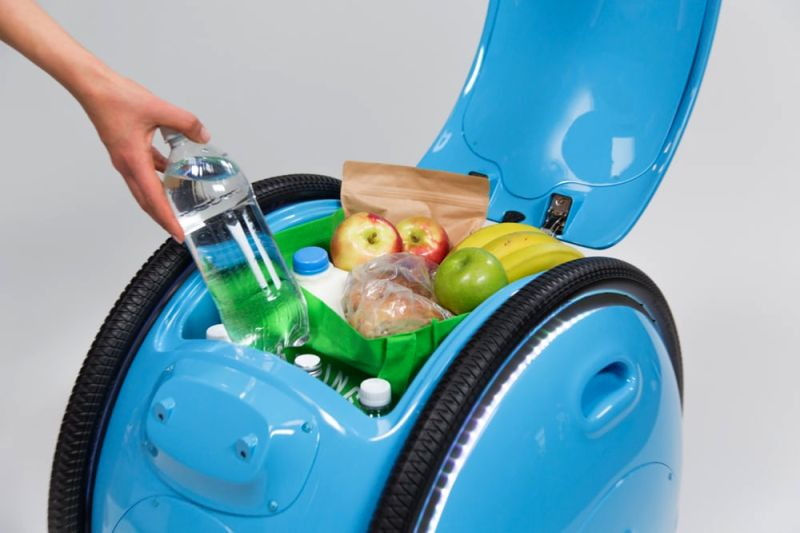
\includegraphics[width = 3.5cm]{img/7.1.jpg}
\label{figura:7.1}
\end{figure}

\subsection{Housekeeper Pro}

\hspace{\parindent}Uma categoria de robô doméstico que faz bastante sucesso é a de limpeza. Existem diversas opções que aspiram o pó no mercado, mas nem todas são fáceis de encontrar. O \textit{Housekeeper Pro}, apesar de ser um bocado caro, está à venda pela \textit{Polishop}. O valor é de 265 euros. Em lojas como \textit{Amazon} e \textit{eBay} há modelos mais baratos e igualmente eficientes \cite{examples}.

\begin{figure}[h]
\caption{Fotografia do \textit{Housekeeper Pro}}
\centering
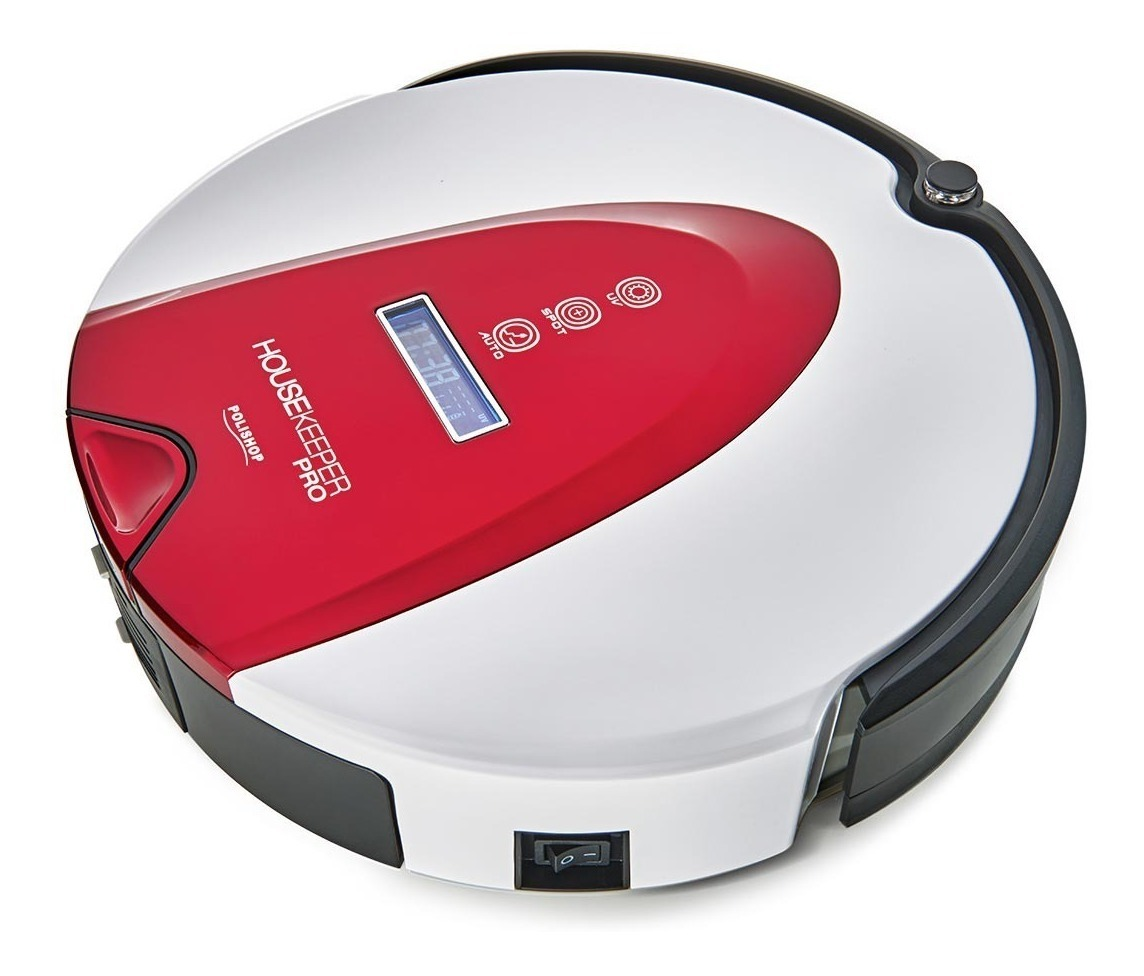
\includegraphics[width = 3.5cm]{img/7.2.jpg}
\label{figura:7.2}
\end{figure}

\subsection{iRobot Braava Jet}

\hspace{\parindent}Quando falamos em limpar a casa, é de conhecimento geral que não adianta apenas tirar o pó, o chão também precisa de ser lavado para ficar tudo limpo. Para isso, existe a linha \textit{iRobot Braava Jet}, que executa essa tarefa como ninguém. Os robôs domésticos da marca iRobot custam mais ou menos 110 euros, cada \cite{examples}.

\begin{figure}[h]
\caption{Fotografia do \textit{iRobot Braava Jet}}
\centering
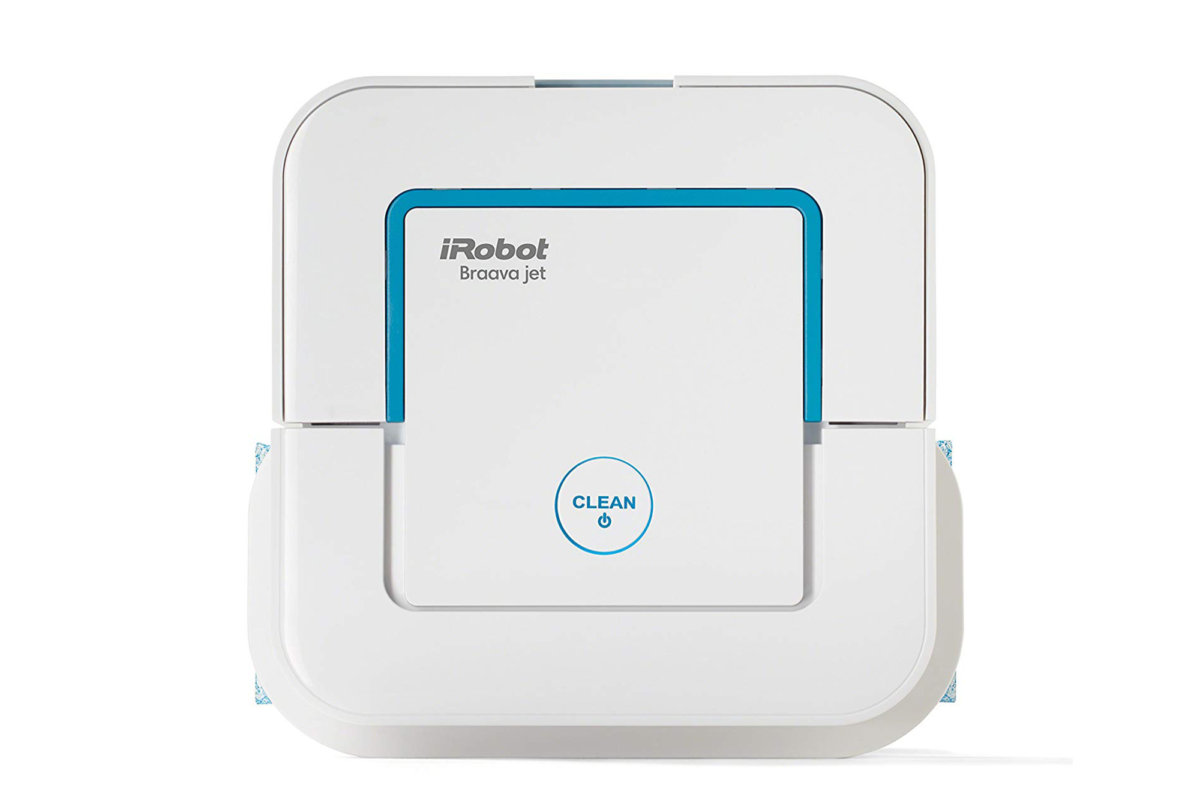
\includegraphics[width = 3.5cm]{img/7.3.jpg}
\label{figura:7.3}
\end{figure}

\subsection{Aibo}

\hspace{\parindent}Durante a CES 2018, uma das maiores feiras de tecnologia \cite{ces}, foi lançado o \textit{Aibo}. Ele não executa nenhuma tarefa física mas faz o papel do seu melhor amigo como ninguém. O robô doméstico em forma de cão tem inteligência artificial, e como tal pode afeiçoar-se a você, pois reconhece rostos e sons. Desenvolvido pela \textit{Sony}, o Aibo funciona a bateria com duração de até duas horas. Por ser um modelo bastante recente, ainda não chegou ao mercado \cite{examples}.

\begin{figure}[h]
\caption{Fotografia do \textit{Aibo}}
\centering
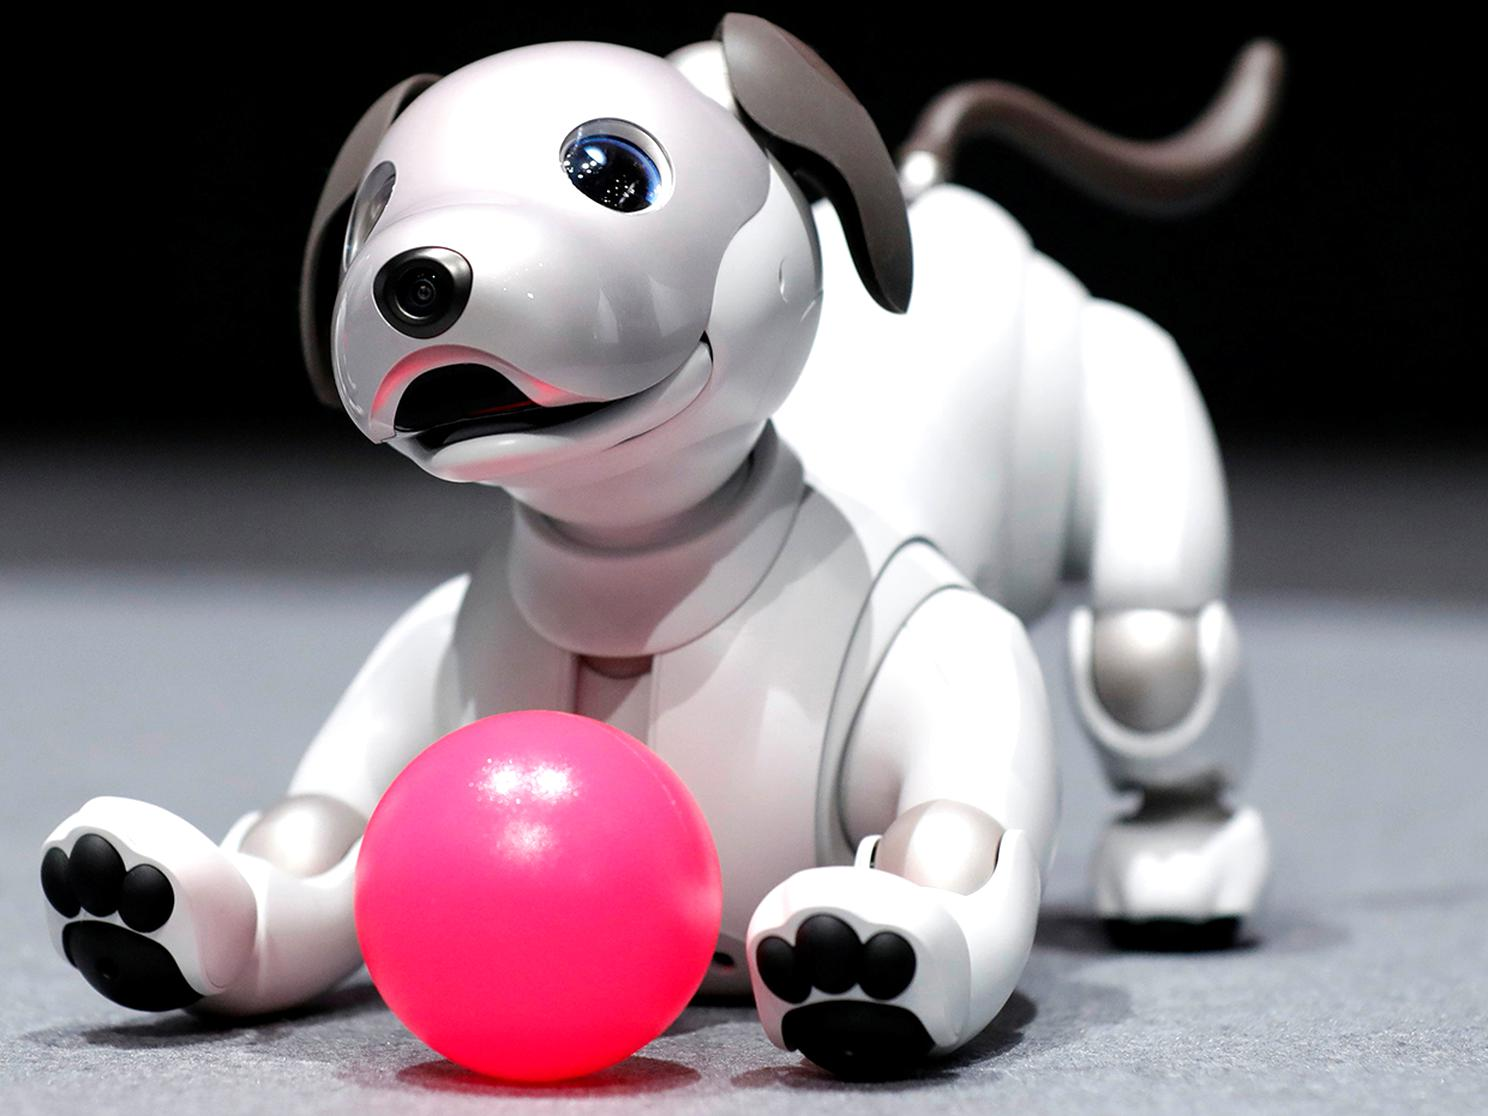
\includegraphics[width = 3.5cm]{img/7.4.jpg}
\label{figura:7.4}
\end{figure}


\subsection{Landroid M}

\hspace{\parindent}Robôs domésticos para cortar a relva também já existem. Como os aspiradores de pó, eles utilizam motores elétricos movidos a baterias recarregáveis. O \textit{Landroid M} tem a funcionalidade de se desviar de canteiros e flores. Essa opção é um pouco mais cara que as restantes mas já está à venda em diversas lojas online. Os preços giram em torno dos 620 euros \cite{examples}.

\begin{figure}[h]
\caption{Fotografia do \textit{Landroid M}}
\centering
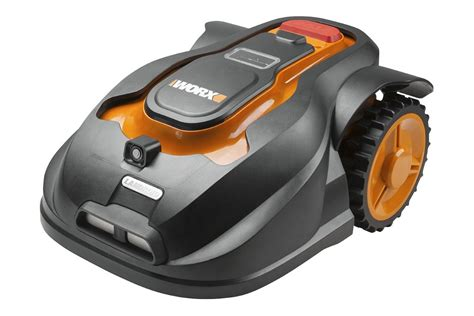
\includegraphics[width = 3.5cm]{img/7.5.jpg}
\label{figura:7.5}
\end{figure}


\section{Segurança na robótica doméstica}

\hspace{\parindent}A segurança não parece ser o ponto forte dos robôs domésticos, nem mesmo daqueles projetados para vigiar as residências dos consumidores. Segundo investigadores da Universidade de Washington, as questões de privacidade e segurança dos utilizadores ainda não receberam a atenção que merecem dos fabricantes desses robôs.

E não se trata de robôs que possam virar-se contra os seus utilizadores e fazer-lhes mal, mas sim de robôs que podem ser controlados por pessoas mal-intencionadas para fins ilegais e prejudicias.
"Tem sido dada muita atenção às questões de tornar os robôs mais inteligentes e de que eles venham a tornar-se perigosos. Mas há um risco muito maior e de curto prazo nomeadamente os robôs a serem utilizados por pessoas mal-intencionadas para fazerem coisas más," explica o investigador Tadayoshi Kohno.

Os riscos associados aos robôs atualmente no mercado, segundo Kohno e os seus colegas, envolvem principalmente o seu funcionamento como uma estação coletora de dados, que podem ser interceptados sem muita dificuldade.

Segundo os investigadores:

A presença do robô é facilmente detectada por mensagens específicas enviadas através da rede sem fios da residência;

Os streams de áudio e vídeo gerados pelo robô podem ser interceptados na rede sem fios e, algumas vezes, pela Internet;

Somente alguns dos robôs analisados emitem um alerta sonoro quando alguém os acessa, informando aos moradores que alguém está a aceder os seus dados;

Somente alguns dos robôs emitem alertas periódicos quando estão a guardar dados.

Os investigadores também identificaram cenários nos quais o robô pode ser utilizado para ferir fisicamente os consumidores ou estragar coisas no ambiente.

Embora os riscos sejam pequenos, os investigadores afirmam que poderão tornar-se mais sérios conforme as capacidades que os robôs adquirem e se disseminem pela maioria das residências.

Uma solução para os problemas destes robôs é a dos seus proprietários ativarem a criptografia da rede sem fios doméstica e desabilitar o acesso ao controle do robô pela internet \cite{security}.


\section{Inovações no ramo da robótica}

\hspace{\parindent}Embora, nos últimos anos, a evolução tenha sido muito acentuada, existe sempre maneira de inovar, e foi com esse intuito que pensámos em algumas ideias:

\begin{itemize}
    \item \textbf{criação de robôs \textit{baby-sitters}:} esta ideia tem prós e contras; a possiblidade de possuir um destes robôs poderia aumentar a empregabilidade de mulheres grávidas, visto que quando estas procuram emprego acabam sempre por nunca ser aceites, o que iria mudar, pois a licença de maternidade das mesmas iria ser menor graças aos tais robôs; em contrário a esta ideia positiva, a manutenção periódica num curto espaço de tempo seria indispensável, já que o robô teria que estar a 100\% (em termos de hardware, e em termos de segurança) para poder assumir tal responsabilidade; 
    \item \textbf{criação de robôs com funcionalidades médicas:} a robótica na medicina não é algo novo, mas esta ideia sim; imaginar robôs domésticos a controlar um ataque de epilepsia, ou até mesmo estabilizar um paciente após um AVC não é muito difícil; com a criação e utilização destes robôs domésticos, a taxa de mortalidade em casa por atraso ou falta de primeiros socorros diminuiria drasticamente, já que os robôs estariam preparados e programados para saber como agir; estes robôs teriam também a possibilidade de fazer vários testes diários ao paciente, tais como medir a febre, pulsação, entre outros.
\end{itemize}

\begin{figure}[h]
\caption{Representação de um robô \textit{baby-sitter} e de um robô médico}
\centering
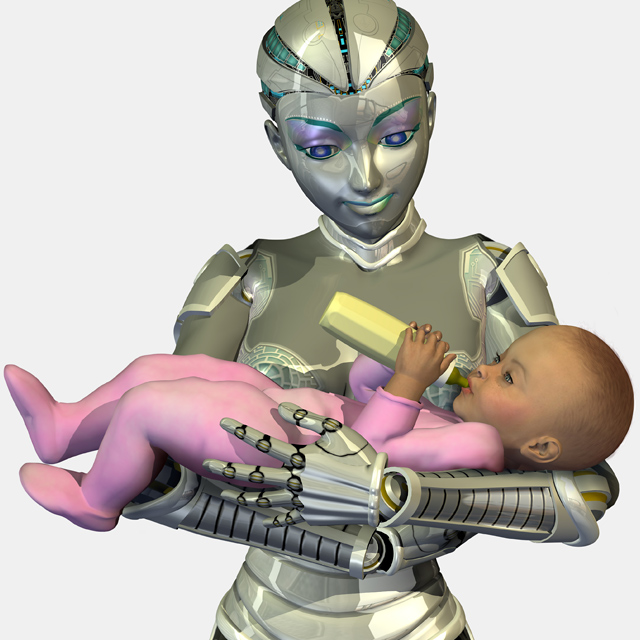
\includegraphics[width = 5cm]{img/9.2.jpg}
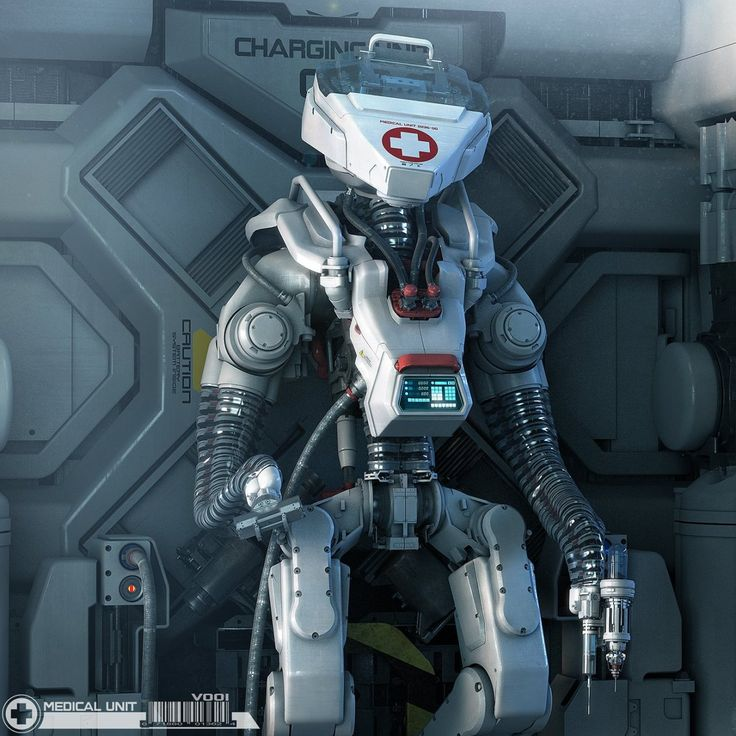
\includegraphics[width = 5cm]{img/9.jpg}
\label{figura:9}
\end{figure}

\newpage

\section{Conclusão}

\hspace{\parindent}Hoje em dia, a robótica doméstica está cada vez mais presente nas nossas vidas e, como tal, é necessário investigar um bocado mais sobre este assunto. Existem muitas variantes às quais é preciso ter atenção antes de avançar com este "projeto", tais como a segurança destes equipamentos, as desvantagens que podem trazer à nossa vida e também o seu custo, visto que alguns destes robôs têm preços elevados. Mesmo que o impacto da evoluções destes robôs tenha tomado proporções gigantes, não podemos pensar que esta parou, até porque todos os dias são feitos novos avanços no ramo da robótica e todos os dias milhares de vidas mudam graças a essa mesma evolução.

\newpage

\printbibliography[title=Referências]

\end{document}
